\vspace{3cm}
\subsubsection{Pagina jocului}

\vspace{1cm}
\begin{center}
	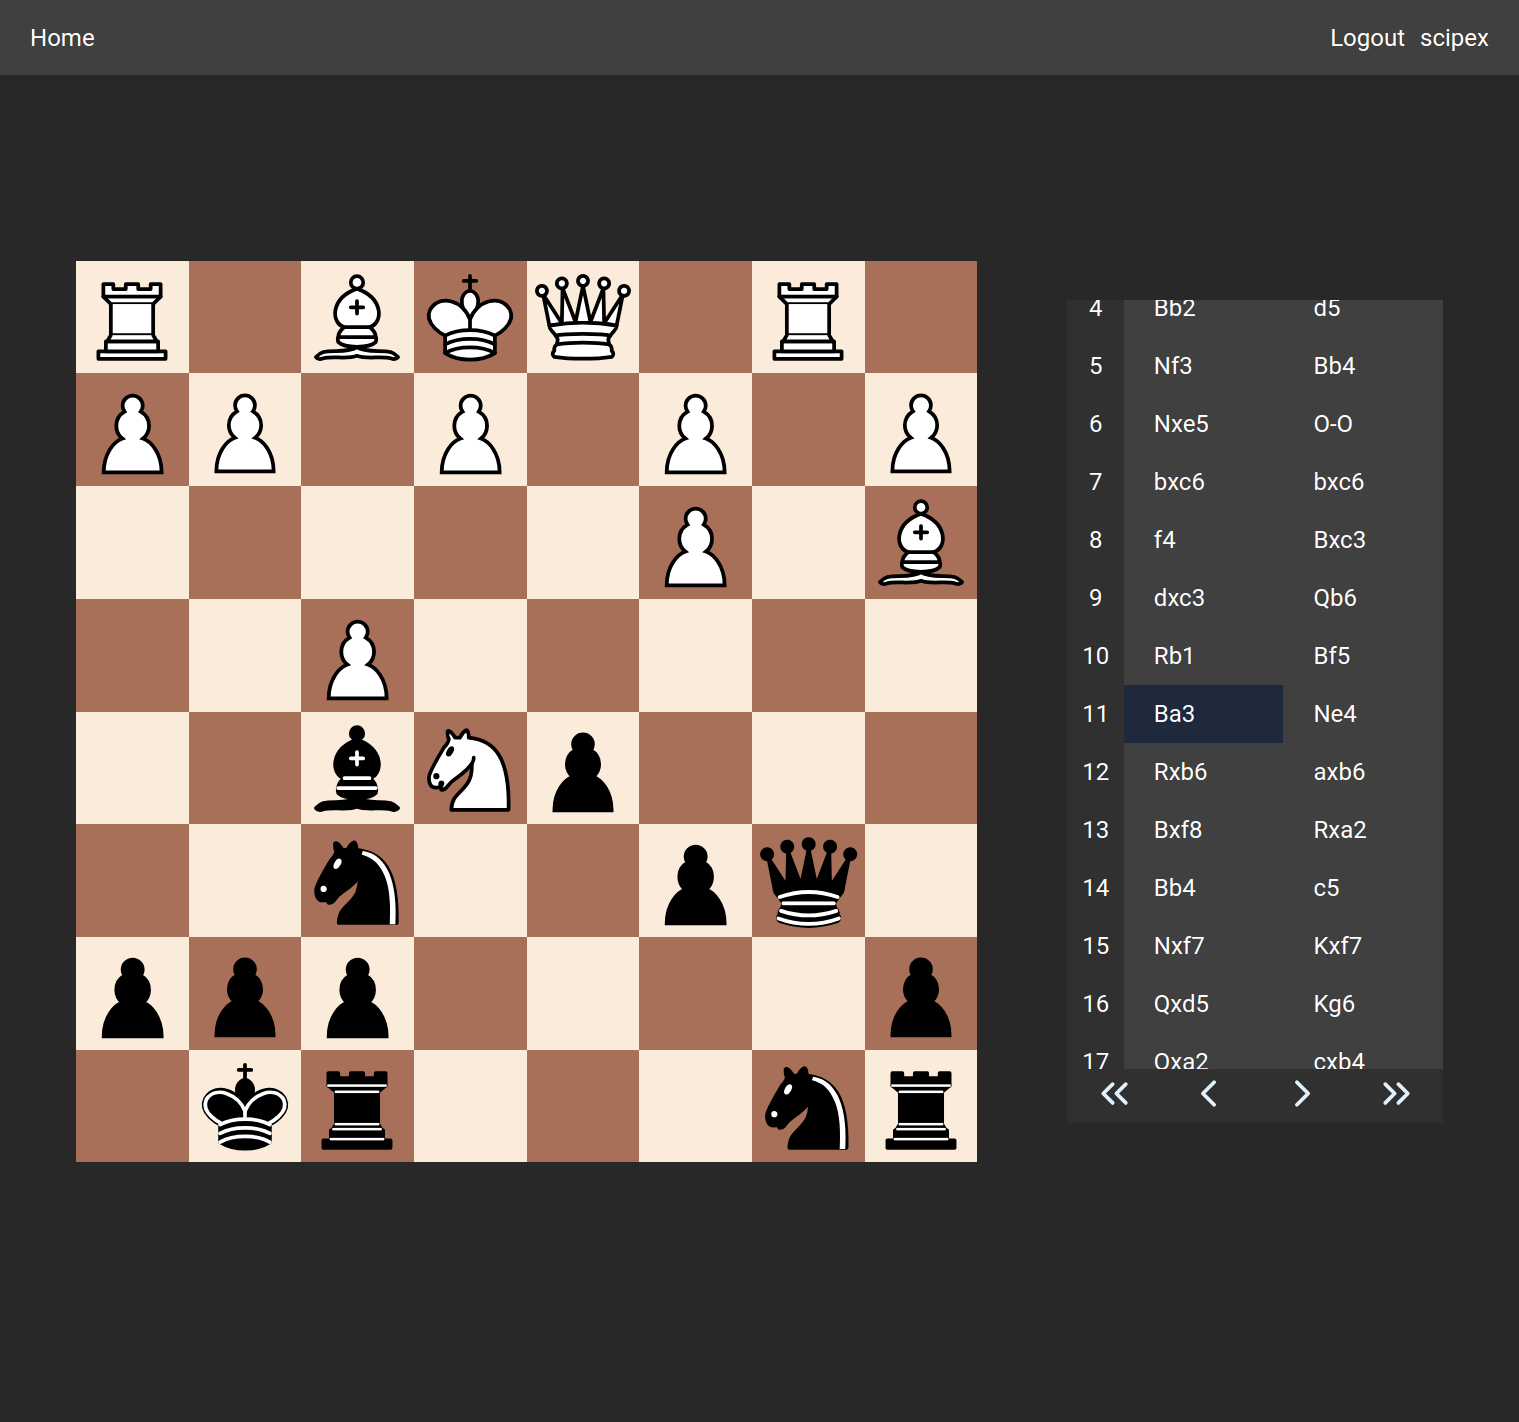
\includegraphics[width=15cm]{3/frontend/game.png}
\end{center}
\vspace{1cm}

Pagina jocului folosește TypeScript și librăria Lit. Este împărțită în 2 secțiuni:

\begin{itemize}

	\item Tabla de joc care interacționează atât la mouse cât și la ecranele tactile
	      \begin{lstlisting}[language=RustHtml]
<div
  class="container"
  @mousedown=${this.mouse_down}
  @mouseup=${this.mouse_up}
  @mousemove=${this.mouse_move}
  @contextmenu=${this.right_click}
>
  ${this.promotion_menu()}
  <div class="board" ${ref(this.board_ref)}>
    ${Array.from(Array(64).keys()).map((i) => this.board_tile(i))}
  </div>
                                                                   
  <div class="piece-hover" ${ref(this.piece_hover_ref)}></div>
</div>


board_tile(i: number) {
  const x = this.flip ? i % 8 : 7 - (i % 8);
  const y = this.flip ? 7 - Math.floor(i / 8) : Math.floor(i / 8);
  const color = (x + y) % 2 == 0 ? "black" : "white";
  const idx = x + y * 8;

  let piece_style = styleMap({});
  if (this.pieces.has(idx)) {
    const p = this.pieces.get(idx)!;

    piece_style = styleMap({
      "background-image": `url(${piece_asset(p.kind, p.color)})`,
      "background-size": "contain",
    });
  }

  return html`<div
    id="tile-${idx}"
    class="tile ${color}"
    style=${piece_style}
    @mouseenter=${(e: MouseEvent) => this.tile_mouseenter(e, idx)}
    @mouseleave=${(e: MouseEvent) => this.tile_mouseleave(e, idx)}
  >
    <div class="legal_move" id="move-${idx}"></div>
  </div>`;
}
 
\end{lstlisting}


	\item Meniul din dreapta care conține lista cu mutări și butoane pentru navigat
	      la începutul jocului, la mutarea precedentă, la mutarea următoare si la ultima
	      mutare, în această ordine

	      \begin{lstlisting}[language=RustHtml]
<div>
  <div class="moves-wrapper" ${ref(this.moves_ref)}>
    <div class="moves">
      ${this.move_pairs().map((pair, i) => this.render_pair(pair, i))}
    </div>
  </div>
  <div class="controls">
    <button class="control" @click=${() => this.handle_ply_select(0)}>
      ${chevron_dleft(30)}
    </button>
    <button
      class="control"
      @click=${() => {
        if (this.drawn_ply > 0) {
          this.handle_ply_select(this.drawn_ply - 1);
        }
      }}
    >
      ${chevron_left(30)}
    </button>
    <button
      class="control"
      @click=${() => {
        if (this.drawn_ply < this.moves.length) {
          this.handle_ply_select(this.drawn_ply + 1);
        }
      }}
    >
      ${chevron_right(30)}
    </button>
    <button
      class="control"
      @click=${() => this.handle_ply_select(this.moves.length)}
    >
      ${chevron_dright(30)}
    </button>
  </div>
</div>


render_pair(pair: MovePair, idx: number) {
  return html`
    <div class="idx">${idx + 1}</div>
    <div
      class=${(this.drawn_ply == idx * 2 + 1 ? "selected" : "") + " white"}
      @click=${() => this.handle_ply_select(idx * 2 + 1)}
    >
      ${move_to_str(pair.white)}
    </div>
    <div
      class=${(this.drawn_ply == idx * 2 + 2 ? "selected" : "") + " black"}
      @click=${() => this.handle_ply_select(idx * 2 + 2)}
    >
      ${pair.black ? move_to_str(pair.black) : ""}
    </div>
  `;
}
\end{lstlisting}

\end{itemize}
